\paragraph*{Contenuto} La pagina, con il pretesto di visitare l'abitazione di Erik e Lars, vuole mostrare le soluzioni del sistema FreedHome propone per le varie zone di casa. L'idea può essere anche valida, ma l'esecuzione è quantomeno discutibile.\\
Bisogna partire dal presupposto che l'utente che naviga su internet ha uno scopo ben preciso, e vuole raggiungere tale scopo nel minor tempo possibile. Nel nostro caso, possiamo supporre che l'utente stia cercando informazioni sui prodotti; sappiamo, inoltre, che in una pagina interna l'utente sosta circa 53 secondi e quindi può leggere un massimo di 159 parole. In questa pagina, contando solamente il corpo dei paragrafi principali, arriviamo 561 parole. Questo problema è aggravato dal contenuto dei paragrafi: la maggior parte di essi non trasmette informazioni utili sui prodotti, ma parla unicamente di Erik e Lars!

\begin{displayquote}
    \textit{Viviamo insieme da 2 anni. E quello che ci tiene insieme è lo spazio aperto che troviamo l’uno
nell’altra. Sì, d’accordo! Capitano anche a noi i momenti dove ognuno si chiude nel proprio
spazio. Il lavoro, la famiglia, le nostre origini ci portano a trovare rifugio in uno spazio
personale. Ma poi prevale la nostra relazione. E così, a volte io, a volte Erika ci apriamo
totalmente per fare passare ciò che in quel momento sentiamo}
\end{displayquote}

Nella pagina, i contenuti validi sono nascosti dietro alla scritta "Entra nella sezione X", che richiede un click da parte dell'utente (male). Si apre quindi una finestra laterale dove finalmente si trova quello che si cerca: a seconda della sezione, si trovano delle foto dettagliate dei prodotti, dei video, e dei paragrafetti che illustrano le caratteristiche dei prodotti; Molto bene.

\begin{figure}
    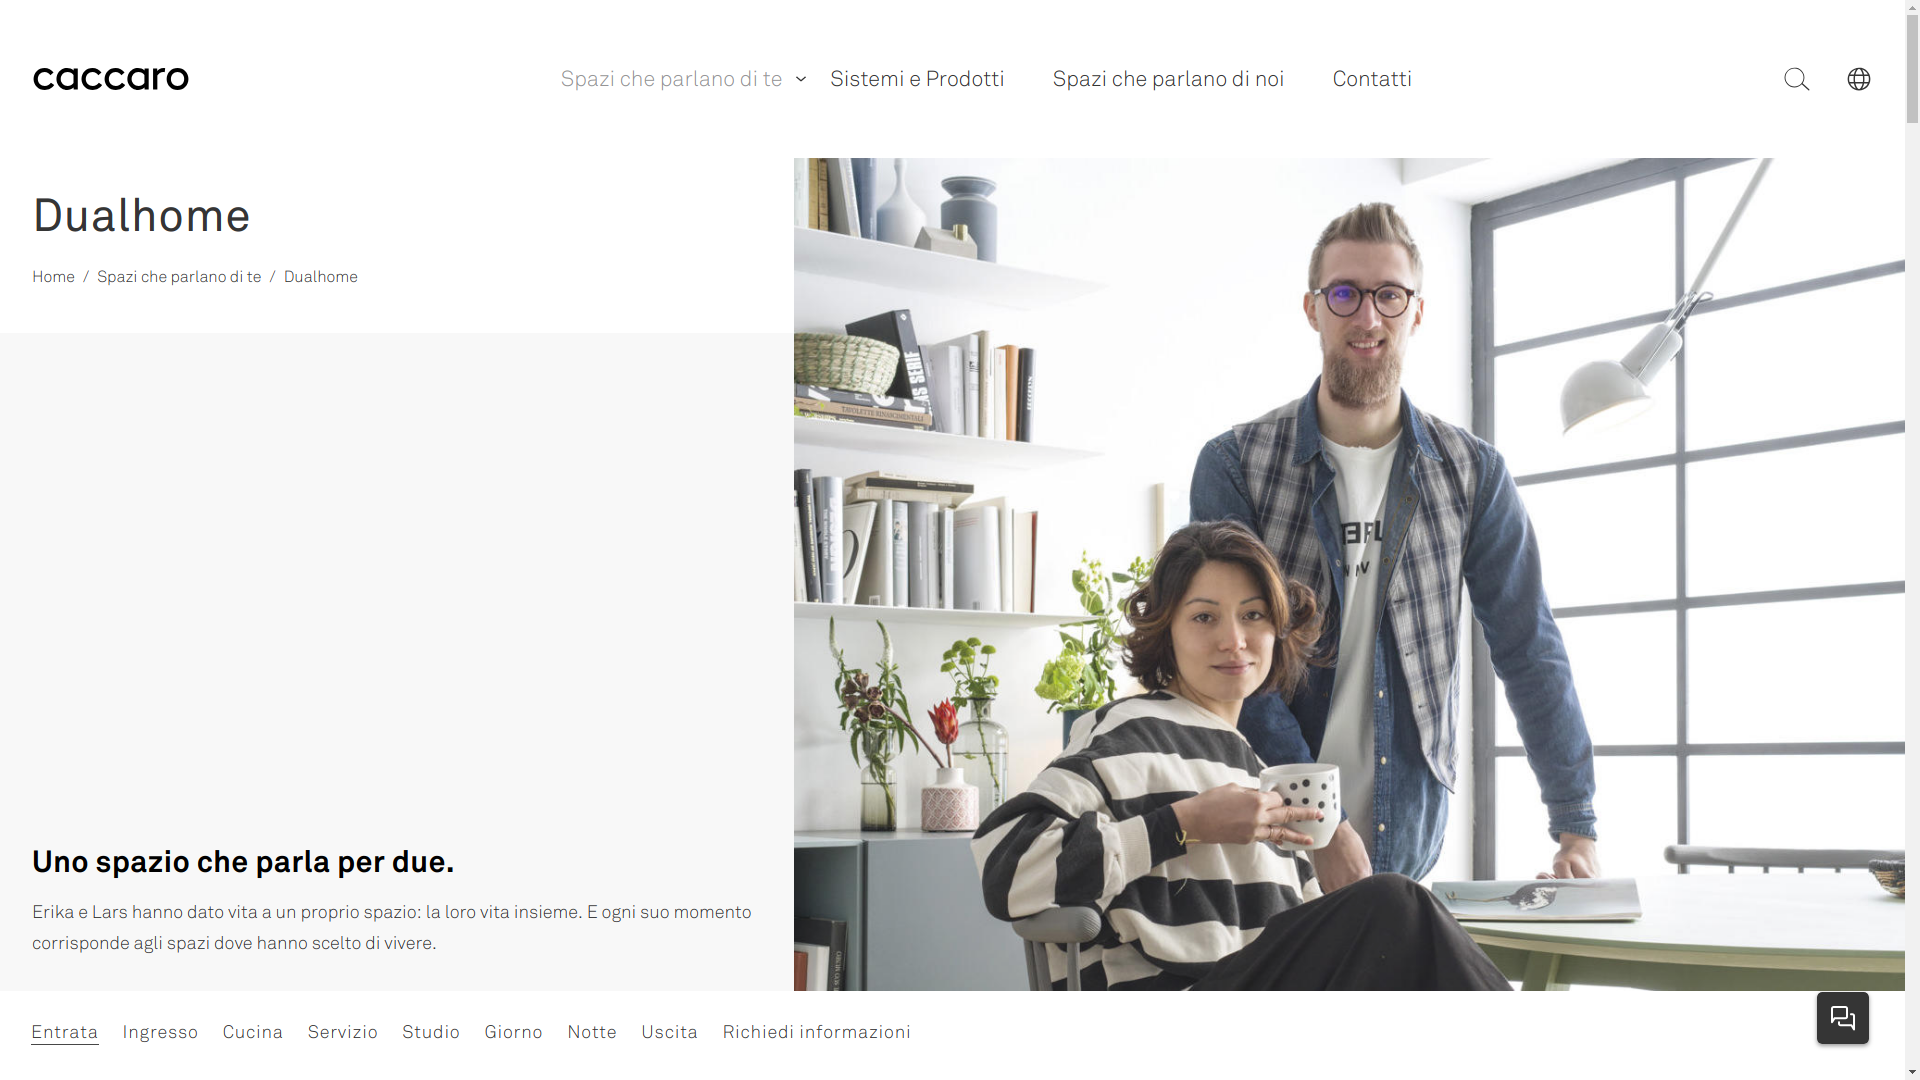
\includegraphics[width=\textwidth]{sez/DualHome/img/main.png}
    \caption{Decisamente troppo eye contact e troppo spazio sprecato.}
    \label{fig:Dual_FirstCut}
\end{figure}

\paragraph*{Video e Immagini}
I video sono un modo per mostrare all'utente contenuto con un basso sforzo computazionale. Nella pagina ne possiamo trovare circa uno per categoria: non superano mai i 40 secondi, e mostrano in modo semplice alcuni dettagli dei prodotti non intuibili da una foto, come l'apertura di un'anta o di un mobile TV. Molto bene.\\
Promosse anche le immagini: sebbene siano sempre incombenti le figure di Erik e Lars, nella maggior parte delle fotografie i prodotti ricevono un'adeguata attenzione. Bene il fatto che la quasi totalità delle immagini sia cliccabile e ingrandibile a pieno schermo. Male la prima immagine, dove i due protagonisti della pagina ci fissano direttamente negli occhi (\autoref{fig:Dual_FirstCut}): lo scopo è quello di farci conoscere la coppia, ma così facendo si distoglie l'utente dalla lettura del testo posto a fianco.

\paragraph*{Scrolling e layout}
\label{sez:DualHome_Scrolling}
Permangono gli stessi problemi affrontati nella home (\fullref{par:Scrolling}): contenuto eccessivo, immagini troppo grandi, e layout rilassato fanno sì che ci siano troppe schermate da scrollare, rendendo quasi inutile il contenuto che si trova nella parte bassa della pagina.
\`E sempre presente un paragrafo che prende tutta la larghezza dello schermo.